%% Copyright 2007-2020 Elsevier Ltd
%% 
%% This file is part of the 'Elsarticle Bundle'.
%% ---------------------------------------------
%% 
%% It may be distributed under the conditions of the LaTeX Project Public
%% License, either version 1.2 of this license or (at your option) any
%% later version.  The latest version of this license is in
%%    http://www.latex-project.org/lppl.txt
%% and version 1.2 or later is part of all distributions of LaTeX
%% version 1999/12/01 or later.
%% 
%% The list of all files belonging to the 'Elsarticle Bundle' is
%% given in the file `manifest.txt'.
%% 
%% Template article for Elsevier's document class `elsarticle'
%% with harvard style bibliographic references
\documentclass[preprint,review,12pt,authoryear]{elsarticle}
\usepackage{amssymb}
\usepackage{amsthm}
\usepackage{amsmath}
\usepackage{caption}
\usepackage[margin=1cm]{geometry}
\journal{Journal of the Mechanics and Physics of Solids}
\begin{document}
\captionsetup[figure]{name={\textbf{Fig.}},labelsep=period} 
\begin{frontmatter}
\title{Inverse design workflow of implicit surface-based cellular materials via conditional generative model and active learning}

\author[1]{Jiaxuan Ma}
\author[3]{Bin Cao}
\author[1]{Yuan Tian}
%\ead{tian0321@shu.edu.cn}
%\author[1]{Yuan Tian\corref{cor1}}
%\ead{tian0321@shu.edu.cn}
\author[3]{Tong-Yi Zhang}
\author[1,2]{Sheng Sun\corref{cor1}}
\ead{mgissh@t.shu.edu.cn}

\address[1]{Materials Genome Institute, Shanghai University, Shanghai, 200444, China}
\address[2]{Shanghai Frontier Science Center of Mechanoinformatics, Shanghai University, Shanghai, 200444, China}
\address[3]{Advanced Materials Thrust, Hong Kong University of Science and Technology (Guangzhou), Guangzhou, 511400, Guangdong, China}

\cortext[cor1]{Corresponding author}

\begin{abstract}
Implicit surface-based cellular materials have attracted considerable interest for bone scaffold applications owing to their structural similarity with natural bone. These materials demonstrate superior mechanical properties and bioadaptability, creating an optimal environment for bone tissue regeneration. However, the rational design of such materials frequently depends on expert knowledge and extensive trial-and-error experimentation. In this study, we present a data-efficient two-stage bi-objective optimization framework within a machine learning paradigm that addresses disparate computational costs between objectives. Applying this methodology to orthopedic implant inverse design, we integrate generative modeling, active learning, and finite element analysis to achieve cellular materials with both biocompatible elastic modulus and enhanced yield strength. Our approach demonstrates substantial performance improvements compared to initial datasets while reducing design costs by approximately sixfold relative to conventional single-step bi-objective optimization methods. This framework establishes an efficient paradigm for rapid intelligent design of cellular materials with tailored mechanical properties, particularly when addressing objectives involving imbalanced computational expenses.
\end{abstract}

\begin{graphicalabstract}
%\includegraphics{grabs}
\end{graphicalabstract}

\begin{highlights}
\item Developed TPMS-GAN with navigator architecture to generate TPMS unit cells satisfying specific mechanical and geometric constraints
\item Created inverse TPMS-GAN for direct design of TPMS unit cells from geometric features, bypassing latent space interpolation or implicit function coefficient adjustment
\item Proposed constraint-aware active learning method to solve bi-objective optimization problems involving objectives with imbalanced computational costs
\end{highlights}

\begin{keyword}
Multi-objective optimization \sep Cellular structure design \sep Generative adversarial network \sep Constraint-aware active learning
\end{keyword}
\end{frontmatter}

\section{Introduction}
Cellular materials have become ubiquitous in engineering applications owing to their exceptional mechanical properties and adaptable characteristics, including lightweight structures \citep{Schaedler2011, Berger2017, Han2015, Tancogne-Dejean2018}, thermal insulation \citep{Li2021d}, acoustic performance \citep{Sekar2024}, and tissue engineering suitability \citep{Li2024c,Peng2023,Tabrizian2024}. The advent of additive manufacturing (AM) has further revolutionized their production by enabling cost-effective fabrication of complex, customized structures. However, despite their broad applicability and potential, the design process for cellular materials remains particularly challenging.

Traditional design methodologies typically employ nature-inspired architectures \citep{Fernandes2021,Bandyopadhyay2021,Sethi2023}, human intuition \citep{Schaedler2011,Berger2017,Xu2016a}, and numerical simulations such as topology optimization \citep{Andersen2019,Bendsoe1999,Collet2018}, spinodal separation \citep{Hsieh2019,Roding2022}, or Gaussian random fields \citep{Kumar2020,Zheng2020abc}. These rule-based approaches are often laborious and time-consuming, with design performance heavily dependent on the designer's expertise.

The emergence of artificial intelligence (AI) has transformed cellular material design paradigms through machine learning. By extracting non-linear relationships between geometric features and mechanical properties from data, trained models can serve as cost-effective surrogates for expensive simulations and experiments. This capability enables seamless integration into heuristic algorithms for optimizing structures with target properties like elastic modulus \citep{Garland2021,Lee2022,Chen2024b}, bulk resistance \citep{Liu2020a}, and stress-strain behavior \citep{Deng2022a,Ma2020b}. However, surrogate optimization requires multiple model invocations, posing challenges for global optimization and real-time design applications.

Generative models including variational auto-encoders (VAE) \citep{Wang2020a,Zheng2023}, generative adversarial networks (GAN) \citep{Nie2020,Shen2022,Kim2020b}, and diffusion models \citep{Bastek2023,Maze2022,Vlassis2023} have demonstrated remarkable potential in cellular material design. These systems learn structural distributions from training data to generate novel configurations. Conditional generative models prove particularly valuable for inverse design challenges where multiple structures correspond to single property targets. Nevertheless, dataset construction costs remain underaddressed, especially in multi-objective scenarios where disparate evaluation costs exist between objectives - a common occurrence when designing cellular structures requiring simultaneous optimization of linear and nonlinear mechanical properties.

Triply periodic minimal surfaces (TPMS), derived from implicit functions with controllable unit cell geometries through coefficient adjustment \citep{Ma2020a}, represent an important class of cellular materials. Characterized by locally symmetric saddle shapes with vanishing mean curvature and non-positive Gaussian curvature, TPMS domains form single connected components without sealed cavities \citep{Kapfer2011}. These geometric properties make them ideal for orthopedic implants where bone-like elastic modulus matching minimizes stress shielding while maximizing yield stress ensures mechanical support and fatigue resistance. Although numerical homogenization efficiently evaluates TPMS elastic modulus, nonlinear plasticity analysis via finite element methods (FEM) incurs substantial computational costs for yield stress determination.

This work presents a two-step strategy combining generative modeling with active learning to address bi-objective TPMS unit cell design involving imbalanced property evaluation costs. As illustrated in Fig \ref{fig:1}, our methodology comprises three components: (1) Generation of structures with target elastic modulus using a trained TPMS-GAN model, creating a virtual design space ($\Omega_E$); (2) Development of an inverse TPMS-GAN (ITPMS-GAN) for latent space exploration and direct geometric manipulation; (3) Elastic modulus-constrained active learning for yield strength optimization. Initial FEM evaluation establishes the dataset, followed by Bayesian optimization (BO)-based active learning \citep{Ma2024b,Cao2024a,Tian2024a} to maximize yield strength within $\Omega_E$. This cohesive workflow seamlessly integrates generative exploration with targeted optimization, enabling the efficient discovery of high-performance TPMS unit cell designs while mitigating computational bottlenecks posed by imbalanced property evaluations.

\begin{figure}
    \centering
    \includegraphics[width=1\linewidth]{figures/1.pdf}
    \caption{\textbf{An overview of the proposed workflow for TPMS unit cells design.} (a) The generator in the TPMS-GAN model produces virtual design space ($\Omega_E$) with desired elastic modulus. (b) The ITPMS-GAN model edits TPMS structures through geometric features to enhance candidate diversity in $\Omega_E$. (c) A machine learning algorithm interactively queries finite element simulations to discover new TPMS designs with high yield strength and target elastic modulus via constrained active learning in $\Omega_E$.}
    \label{fig:1}
\end{figure}

\section{Models and methods}
\subsection{TPMS-based cellular structures}
TPMS can be generated using a level-set approximation equation expressed as a sum of Fourier series terms [xxx]:
\begin{equation}
 \Psi(\boldsymbol{r})=\sum_kF(\boldsymbol{k})\cos\left([2\pi \boldsymbol{k}\cdot \boldsymbol{r}-\alpha(\boldsymbol{k})]\right)=0
\label{eq:1}
\end{equation}
where $\boldsymbol{k}$ represents the reciprocal vector, $\alpha(\boldsymbol{k})$ denotes a phase shift, and $F(\boldsymbol{k})$ corresponds to the amplitude associated with the given $\boldsymbol{k}$ vector. When truncated to the leading term, this series produces a function $\phi$ composed of trigonometric combinations satisfying $\phi(\boldsymbol{r})=\phi(x,y,z)=c$. The surface defined by $\phi(x, y, z)$ at isovalue $c$ exhibits topological similarity to minimal surfaces.

\subsection{Effective properties of homogenized cellular structures}
\label{subsec:homo}
This study employs a voxel-based asymptotic homogenization method \citep{Dong2019} to calculate the effective elastic tensor of TPMS unit cells. The method assumes physical quantities like stress and strain depend on both macroscale ($X$) and microscale ($x/\varepsilon$), where $\varepsilon$ represents the scale factor. These quantities are homogenized at the macroscale while maintaining periodicity at the microscale. By asymptotically expanding the microscopic strain tensor and neglecting higher-order terms, we obtain:
\begin{equation}
    \varepsilon = \bar{\varepsilon} + \varepsilon^{*}
\label{eq:2}
\end{equation}
Here, $\bar{\varepsilon}$ signifies macroscopic mean strain within the unit cell, while $\varepsilon^{*}$ indicates periodic microscale perturbation strain. The perturbation strain is obtained by solving the mechanical balance equation:
\begin{equation}
\int_{\Omega}\hat{\varepsilon}^T:\mathbb{C}:\varepsilon^{*}d\Omega = \int_{\Omega}\hat{\varepsilon}^T:\mathbb{C}:\bar{\varepsilon}d\Omega
\label{eq:3}
\end{equation}
where $\hat{\varepsilon}$ represents virtual strain, $\mathbb{C}$ the material elastic tensor, and $\Omega$ the unit cell domain. This equation is numerically discretized using finite element analysis with eight-node hexahedrons, voxelizing each unit cell into $40 \times 40 \times 40$ cubes (Fig S1). Following determination of $\varepsilon^{*}$, the effective elastic tensor $\mathbb{C}^H$ becomes:
\begin{equation}
\mathbb{C}^H:\bar{\varepsilon} = \frac{1}{|\Omega|}\int_{\Omega}\mathbb{C}:(\bar{\varepsilon}+\varepsilon^{*})d\Omega
    \label{eq:4}
\end{equation}
where $|\Omega|$ denotes unit cell volume.

Elastic modulus $E_{ijk}$ along the $[i,j,k]$ direction can be calculated using the following equation:
\begin{equation}
\frac{1}{E_{ijk}} = \mathbb{S}^H_{11} - 2 \left(\mathbb{S}^H_{11} - \mathbb{S}^H_{12} - \frac{1}{2} \mathbb{S}^H_{44} \right) \times \left( \ell_{i1}^2 \ell_{j2}^2 + \ell_{j2}^2 \ell_{k3}^2 + \ell_{i1}^2 \ell_{k3}^2 \right),
    \label{eq:6}
\end{equation}

where $\ell$ is the cosine of the angle between the orientation $[i,j,k]$ and the coordinate axes $[x, y, z]$, and $\mathbb{S}^H$ the compliance tensor with $\mathbb{S}^H = (\mathbb{C}^H)^{-1}$.  This formulation enables graphical representations of the variation in the magnitude of $E_{ijk}$ with respect to the crystallographic axes (Fig S1).

\subsection{The architecture of TPMS-WGAN model}
In this work, we implement a conditional Wasserstein GAN consisting of four key components: a generator network ($G_\phi$), a discriminator network ($D_\theta$), a navigator network ($R_\omega$), and a condition module $\boldsymbol{C}$ incorporating mechanical properties and geometric features of the TPMS unit cell. Individual conditions can be selectively activated or deactivated during training to accommodate diverse design requirements (Fig. \ref{fig:2}). The generator $G_\phi$, parameterized by trainable weights $\phi$, transforms Gaussian noise ($\boldsymbol{z}$) and conditional inputs into TPMS structural parameters $\boldsymbol{p} \in \mathbb{R}^4$, producing synthetic outputs $\boldsymbol{p}'$. Simultaneously, the discriminator $D_\theta$ with parameters $\theta$ evaluates the authenticity of input parameter sets. It accepts real data $\boldsymbol{p}$, generated samples $\boldsymbol{p}'$, and conditional inputs $\boldsymbol{C}$, outputting a scalar value $D_\theta(\boldsymbol{p}'|\boldsymbol{C})$ that quantifies the realism of generated parameters.

The adversarial training process establishes a two-player minimax game between generator and discriminator, formalized by the loss function:

\begin{equation}
\mathcal{L}_{(G_\phi, D_\theta)}= \min_G \max_{D} \mathbb{E}_{\boldsymbol{p} \sim \mathbb{P}_r} \left[ D_\theta(\boldsymbol{p}|\boldsymbol{C}) \right] - \mathbb{E}_{\boldsymbol{p}' \sim \mathbb{P}_g} \left[ D_\theta (\boldsymbol{p}') \right]
\label{eq:7}
\end{equation}

where $D$ represents 1-Lipschitz functions, $\mathbb{P}_r$ denotes the data distribution, and $\mathbb{P}_g$ corresponds to the implicit model distribution defined by $\boldsymbol{p}'=G_\phi(\boldsymbol{z}|\boldsymbol{C})$. To stabilize training dynamics and address gradient-related challenges, we implement Wasserstein GAN with gradient penalty (WGAN-GP) \citep{Gulrajani2017}.

\begin{figure}
    \centering
    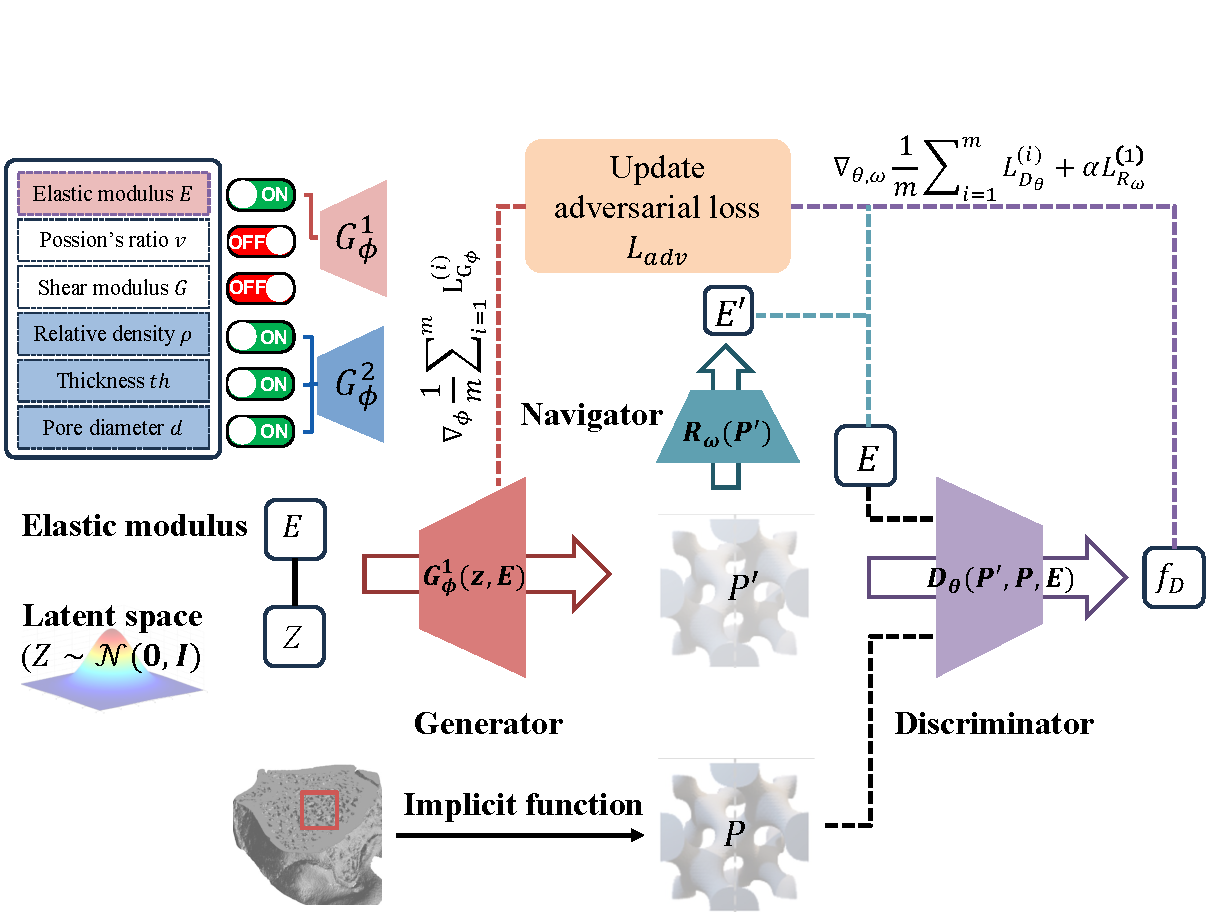
\includegraphics[width=1\linewidth]{figures/3.pdf}        
    \caption{\textbf{Generative modeling framework}. Our conditional WGAN architecture, termed TPMS-WGAN, integrates multiple mechanical and geometric conditions for TPMS unit cell design. Conditions can be independently toggled during training. For elastic modulus integration, the model combines effective modulus $E$ with Gaussian noise $\boldsymbol{z} (\boldsymbol{z}\sim\mathcal{N}(\mathbf{0},\mathbf{I}))$ as generator inputs. The synthesized structural parameters $\boldsymbol{p}'$, along with real data $\boldsymbol{p}$ and modulus $E$, are fed to the discriminator for realism assessment ($f_D$). Concurrently, generated parameters undergo navigator network processing to predict elastic modulus $E'$.}
    \label{fig:2}
\end{figure}

\subsection{Constraint-aware active learning}
\label{sec:2-4}
Bayesian optimization (BO)-based active learning methods excel in solving computationally expensive black-box problems. Unlike gradient-based or heuristic approaches that rely solely on surrogate model predictions, BO leverages probabilistic estimates from sequentially updated surrogate models. The framework comprises two core elements:
\begin{itemize}
    \item A surrogate model enabling efficient exploration of virtual design spaces with uncertainty quantification
    \item An acquisition function (AF) balancing exploration and exploitation to score candidate samples
\end{itemize}

We employ support vector machines (SVM) as surrogates for expensive finite element simulations of TPMS yield strength. Bootstrap methods introduce prediction uncertainties, constructing the probabilistic model:
$$
y=f(\boldsymbol{x})+\varepsilon,\quad \varepsilon\sim(0, \Sigma^2)
$$
This model estimates mean predictions $f(\boldsymbol{x})$ and associated uncertainties $\Sigma^2$ across unexplored design spaces.

BO operates through iterative optimization cycles. At each iteration:
\begin{enumerate}
    \item SVM evaluates all unobserved samples in $\Omega_E$
    \item AF selects optimal candidate $\hat{\boldsymbol{x}}^*$ for simulation/experimentation
    \item New data pair $(\hat{\boldsymbol{x}}^*, f(\hat{\boldsymbol{x}}^*))$ augments dataset $\mathcal{D} = \{(\boldsymbol{x}_1, f(\boldsymbol{x}_1)), \ldots, (\boldsymbol{x}_n, f(\boldsymbol{x}_n))\}$
    \item SVM updates to improve predictive accuracy
\end{enumerate}

The process iterates until meeting convergence criteria or budget limits. Central to this approach is AF-driven candidate selection via expected utility maximization:

\begin{equation}
\alpha(\boldsymbol{x}) = \mathbb{E}[I(\boldsymbol{x})|\mathcal{D}]
\label{eq:8}
\end{equation}

Using the prevalent Expected Improvement (EI) utility function:
\begin{equation}
I_\text{EI}(\boldsymbol{x})=\max(f(\hat{\boldsymbol{x}})-f^*, 0)
\label{eq:9}    
\end{equation}

Substituting into Eq. \ref{eq:8} and applying reparameterization yields:
\begin{equation}
\alpha_\text{EI}(\boldsymbol{x}) = \left(\mu(\boldsymbol{x}) - f^*\right) \Phi\left(\frac{\mu(\boldsymbol{x}) - f^*}{\Sigma(\boldsymbol{x})}\right) + \Sigma(\boldsymbol{x}) \phi\left(\frac{\mu(\boldsymbol{x}) - f^*}{\Sigma(\boldsymbol{x})}\right)
\label{eq:10}    
\end{equation}

where $\phi(\cdot)$ denotes the probability density function (PDF) and $\Phi(z)$ represents the cumulative distribution function (CDF) of the standard normal random variable $z$. The right-hand side consists of two components: the first term governs exploitation, while the second facilitates exploration. The acquisition function evaluates unknown samples in the virtual design space to identify potential candidates for subsequent simulations or experiments.

The incorporation of inequality constraints into Bayesian optimization can be formulated as:
\begin{equation}
\max_{c(\boldsymbol{x}) \leq \lambda} f(\boldsymbol{x})
\label{eq:11}
\end{equation}
where $c(\boldsymbol{x})$ represents additional outputs from dataset $\mathcal{D}$, modeled independently through a probabilistic framework analogous to $f(\cdot)$. The constraint $c(\boldsymbol{x})\leq \lambda$ defines the feasible region within the virtual design space. The constrained expected improvement for candidate $\hat{\boldsymbol{x}}$ is expressed as:
\begin{equation}
I_{\text{EI-C}}(\hat{\boldsymbol{x}})=\Delta_\text{C}(\hat{\boldsymbol{x}})\max\{0, f(\hat{\boldsymbol{x}})-f^*\}=\Delta_\text{C}(\hat{\boldsymbol{x}})I_{\text{EI}}(\hat{\boldsymbol{x}})
    \label{eq:12}
\end{equation}
where $\Delta_\text{C}(\hat{\boldsymbol{x}})\in \{0,1\}$ serves as a feasibility indicator, equaling 1 if $c(\hat{\boldsymbol{x}})\leq \lambda$ and 0 otherwise. This binary random variable follows a Bernoulli distribution:
\begin{equation}
    PF(\hat{\boldsymbol{x}}):=Pr[c(\boldsymbol{x})\leq \lambda] 
    \label{eq:13}
\end{equation}
Here, $PF(\hat{\boldsymbol{x}})$ corresponds to the cumulative distribution function. These derivations culminate in the constrained expected improvement acquisition function:
\begin{equation}
\begin{aligned}
\alpha_{\text{EI-C}}(\hat{\boldsymbol{x}}) &=\mathbb{E}[I_\text{EI-C}(\hat{\boldsymbol{x}})]\\
&= \mathbb{E}[\Delta_{C}(\hat{\boldsymbol{x}})I_{\text{EI}}(\hat{\boldsymbol{x}})|\hat{\boldsymbol{x}}]\\
&= \mathbb{E}[\Delta_{C}(\hat{\boldsymbol{x}})|\hat{\boldsymbol{x}}]\mathbb{E}[I_\text{EI}(\hat{\boldsymbol{x}})|\hat{\boldsymbol{x}}]\\
&=PF(\hat{\boldsymbol{x}})\alpha_{\text{EI}}(\hat{\boldsymbol{x}})
\end{aligned}
\label{eq:14}
\end{equation}

Thus, $\alpha_{\text{EI-C}}(\hat{\boldsymbol{x}})$ represents the standard expected improvement weighted by the feasibility probability of $\hat{\boldsymbol{x}}$. In our methodology, we substitute $PF(\hat{\boldsymbol{x}})$ with a normalized distance metric between constraint value $c(\hat{\boldsymbol{x}})$ and target point $c^*$, denoted as $ND(||c(\hat{\boldsymbol{x}})-c^*||)$. This modification adaptively adjusts the distribution of $\alpha_{\text{EI}}(\hat{\boldsymbol{x}})$ without requiring additional probabilistic modeling for constraints. Consequently, Equation \ref{eq:14} transforms into:
$\alpha_{\text{EI-C}}(\hat{\boldsymbol{x}}) =ND(||c(\hat{\boldsymbol{x}})-c^*||)\alpha_{\text{EI}}(\hat{\boldsymbol{x}})$. 

Figure \ref{fig:6} contrasts constraint-unaware and constraint-aware active learning processes. The blue dot in Fig. \ref{fig:6}\textbf{a} marks the optimum for the unconstrained objective function, while the red dot in Fig. \ref{fig:6}\textbf{b} indicates the constrained counterpart. Our normalized constraint function modifies EI scores across the virtual data space, evident in the shifted query points from Fig. \ref{fig:6}\textbf{c} to \ref{fig:6}\textbf{d} (see Supplementary Note S3). This approach successfully identifies optimal points under constraints and influences subsequent query selection through exploitation-exploration balance adjustments.

\section{Results and Discussions}
\subsection{Database of TPMS-based cellular structures}

Schoen's gyroid (G) and diamond (D) TPMS configurations exhibit remarkable geometric versatility with an exceptionally broad elastic modulus range \citep{Lee2016}. Their implicit functions $f(x,y,z)$ are defined as:

\begin{equation}
\begin{aligned}
f_G(x,y,z)&= \cos(2\pi y)\sin(2\pi x)+\cos(2\pi x)\sin(2\pi z)\\&+\cos(2\pi z)\sin(2\pi y)+t_1 = 0, t_1 =0
\end{aligned}
\label{eq:15}
\end{equation}
\begin{equation}
\begin{aligned}
f_D(x,y,z)&=\cos(2\pi x)\cos(2\pi y)\cos(2\pi z)\\&-\sin(2\pi x)\sin(2\pi y)\sin(2\pi z)+t_2=0, t_2 =0
\end{aligned}
\label{eq:16}
\end{equation}

Beyond their compact representations, TPMS-based units can be diversified through function combinations and coefficient adjustments \citep{Wang2019b}. Our hybrid structures combine G and D configurations via weighted implicit functions:
\begin{equation}
\begin{aligned}
    f_{Hybrid}(x, y, z) &=\alpha_1 (4f_G(x,y,z))+\alpha_2(4f_D(x, y,z ))\\
    \alpha_1+\alpha_2 &= 1,
    0\leq\alpha_1, \alpha_2 \leq1,
\end{aligned}
\label{eq:17}
\end{equation}

Parameters $\alpha_1$ and $\alpha_2$ vary stochastically while maintaining unit summation to generate structural diversity. Level set values  {不一致}{$t_1$ and $t_2$}, constrained within [-0.5, 0.5], control volume fractions through surface thickness modulation. Variations in $\alpha_1, \alpha_2, t_1,$ and $t_2$ (Eq.\ref{eq:17}) produce distinct TPMS architectures as depicted in Fig. \ref{fig:3}. These amalgamations induce both geometric variations and mechanical property modifications in TPMS unit cells.


We constructed a comprehensive database of TPMS unit cells by perturbing parameters $\{\alpha_1, \alpha_2, t_1, t_2\}$ through Latin hypercube sampling (LHS), generating 1372 unique structures after excluding invalid configurations. These structures demonstrate isotropic mechanical properties arising from the cubic symmetry inherent to merged TPMS unit cells. For each structure, we calculated the effective mechanical stiffness tensor using numerical homogenization methods as described in Section \ref{subsec:homo}. The mechanical behavior of cellular materials depends on both scaffold architecture and constituent material properties.

Ti6Al4V (Ti) alloy was selected as the constituent material for orthopedic implants \citep{Peng2023}, with material parameters detailed in Table S1. Widely adopted for 3D-printed bone defect repairs, this bio-inert Ti alloy has achieved clinical success in medical applications. Figure \ref{fig:2}b illustrates the distributions of effective elastic modulus ($E$) and Poisson's ratio ($v$) for G, D, and hybrid TPMS unit cells. Notably, we evaluated an additional 100 samples for G and D structures beyond the primary dataset. The Poisson's ratio distributions for G and D exhibit single-curve patterns inversely correlated with relative density, while hybrid TPMS configurations show broader property variations.

The relationship between effective elastic modulus $E$ and relative density $\rho$ follows the exponential form:
$$E \propto E_s\rho^{n}$$
as established in prior research \citep{Bauer2017}, with additional details provided in Supplementary Note S1.

\begin{figure}
    \centering
    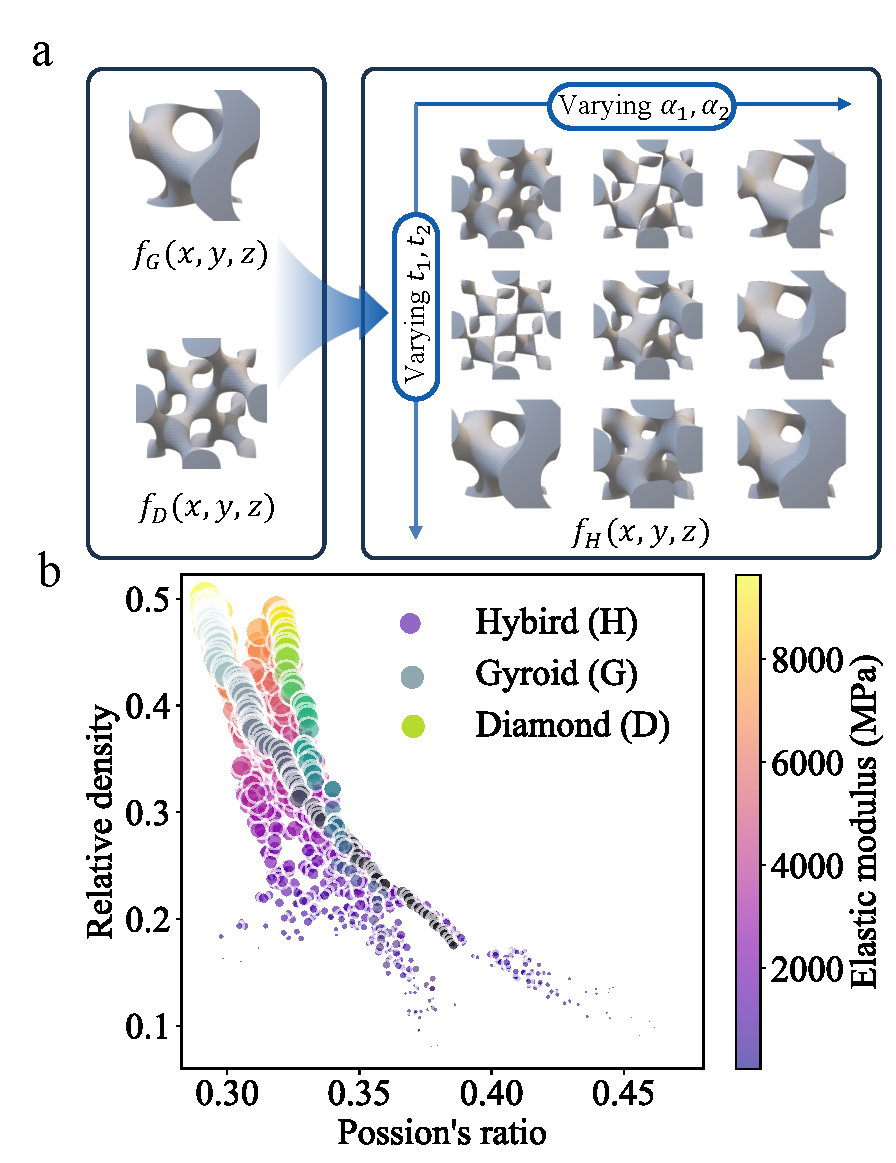
\includegraphics[width=0.75\linewidth]{figures/2.pdf}
    \caption{\textbf{Structural variations and property distributions of merged TPMS unit cells}. \textbf{a} Representative structures generated by varying shape parameters $\alpha_1, \alpha_2,t_1,t_2$ for Gyroid (G) and Diamond (D). \textbf{b} Dataset visualization of effective elastic modulus $E$, Poisson's ratio $v$, and relative density $\rho$ using plasma colormap. Marker sizes correlate with $E$. Property variations for G and D structures were evaluated through incremental $t_i( i=1,2,\Delta t = 0.01$) adjustments within $f_G$ and $f_D$, each analyzed across 100 samples (represented by bone and viridis colormaps).}
    \label{fig:3}
\end{figure}

\subsection{Performance of TPMS-WGAN}
To train the TPMS-GAN for generating virtual designs with target elastic moduli, we implemented conditional training focused on $E$ while disabling other constraints. The hybrid TPMS dataset was partitioned into 1098 training and 274 testing samples (8:2 ratio). Input parameters $\alpha_1, \alpha_2$, and $E$ were normalized prior to network input, with architecture details provided in Table S5.

We enhanced generative performance by ensuring accurate parameter-to-property mapping through a dedicated property navigator $R_\omega$. This introduced an additional loss term:
\begin{equation}
\mathcal{L}_{(R_\omega)}=\mathbb{E}_{\boldsymbol{p}' \sim \mathbb{P}_g}(|R_\omega(\boldsymbol{p}')-E|)
\label{eq:18}
\end{equation}

The combined discriminator loss becomes:
\begin{equation}
\mathcal{L}_{D_\theta} =  \mathcal{L}_{(G_\phi, D_\theta)} + \eta *\mathcal{L}_{R_\omega}
\label{eq:19}
\end{equation}
where $\eta=0.5$, with generator loss defined as:
\begin{equation}
\mathcal{L}_{G_\phi} =  - \mathbb{E}_{\boldsymbol{z}\sim \mathcal{N}(\boldsymbol{0},\boldsymbol{I})} \left[ D_\theta (G_\phi(\boldsymbol{z}|\boldsymbol{C})\right]
\label{eq:20}
\end{equation}

Figure \ref{fig:4} compares navigator-free and navigator-enhanced TPMS-WGAN architectures. The navigator generator demonstrates superior training stability (blue vs green curves in Fig. \ref{fig:4}a) with lower discriminator losses (2.57 vs 3.12). t-SNE and KSFE visualizations (Fig. \ref{fig:4}c,d) reveal closer alignment between navigator-generated data and training distributions.

Wasserstein distance calculations \citep{Villani2008OptimalTO} quantify this improvement, showing distances of 0.34 (navigator-free) versus 0.23 (navigator-enhanced). Random forest evaluations (Fig. \ref{fig:4}e,f) demonstrate enhanced agreement between generated and test data elastic moduli ($R^2=0.982$ vs $0.706$), confirming the navigator's effectiveness in guiding gradient descent during training.

\begin{figure}
    \centering
    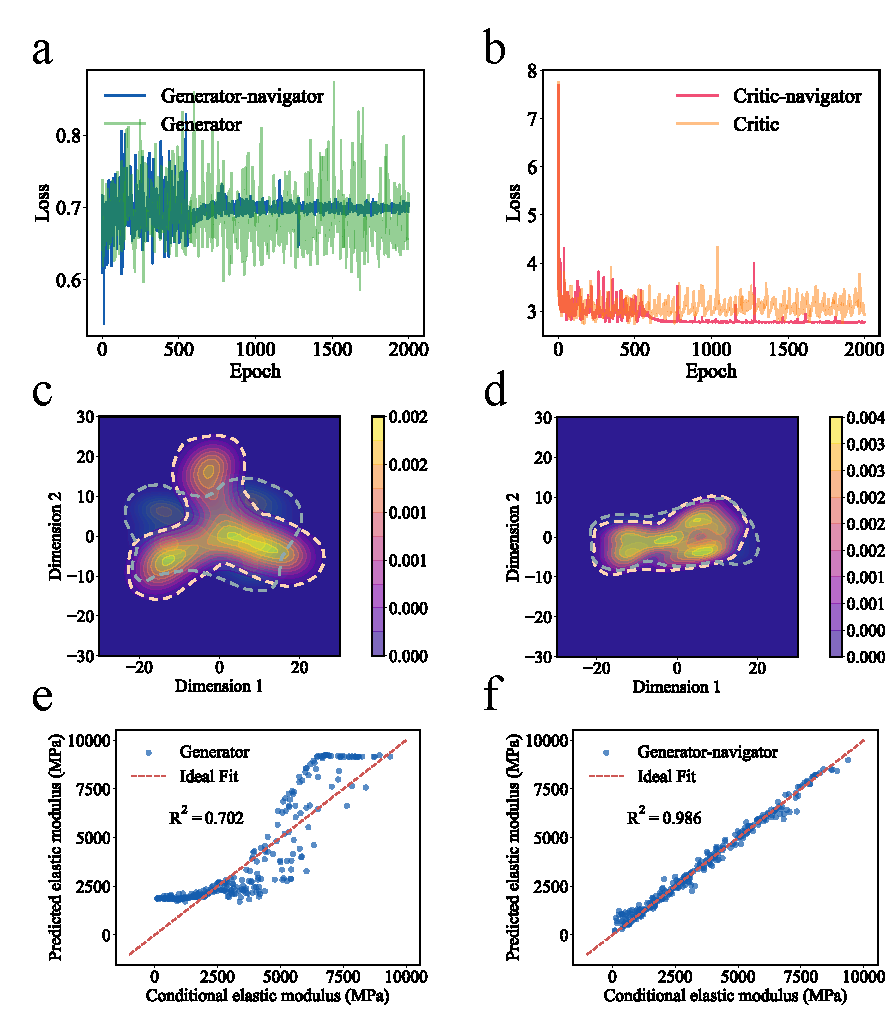
\includegraphics[width=0.75\linewidth]{figures/4.pdf}
    \caption{\textbf{Evaluation of the TPMS-GAN model.} (\textbf{a}) Loss values for the navigator-free generator (green) and navigator generator (blue) during training. (\textbf{b}) Loss values for the navigator-free discriminator (orange) and navigator discriminator (red). 2D t-SNE plots show data distributions: training data (viridis colormap) versus generated data (plasma colormap) under corresponding elastic moduli for navigator-free generator (\textbf{c}) and navigator generator (\textbf{d}). Density represents probability per unit area. Conditional vs evaluated elastic moduli comparisons for structures from the navigator-free generator (\textbf{e}) and navigator generator (\textbf{f}).}
    \label{fig:4}
\end{figure}

The continuous, low-dimensional latent space with generative capabilities enables efficient structural design through arithmetic operations on latent representations ($\boldsymbol{z}$). However, conditional WGANs cannot map real structures to their latent spaces. To overcome this limitation, we trained an encoder $IG_\psi$ to approximate the inverse mapping $(\boldsymbol{z},\boldsymbol{C})=IG_\psi(\boldsymbol{p})$. This allows derivation of latent representations $\boldsymbol{z}$ from real TPMS structures $\boldsymbol{p}$, facilitating latent space exploration via interpolation or other transformations.

While existing generative models for cellular materials successfully map topology and mechanical properties to latent spaces, they lack explainability in manipulating TPMS unit cell geometry through latent variables or implicit function coefficients. Our proposed inverse TPMS-GAN (ITPMS-GAN) integrates a trained TPMS-GAN: once $\boldsymbol{z}$ is obtained from structure parameters $\boldsymbol{p}$, explicit geometric control can be applied via conditions. In this framework, the encoded latent space $\boldsymbol{z}'$ and edited geometry condition $\bar{\boldsymbol{s}}$ serve as inputs to the generator, producing new TPMS unit cells with parameters $\boldsymbol{p}'$.

We trained $IG_\psi$ post-TPMS-GAN training using both original ($\boldsymbol{p}$) and generated ($\boldsymbol{p}'$) parameters. The reconstruction loss is minimized through:

\begin{equation}
    \mathcal{L}_{IG} = \frac{1}{m}\sum_{i=1}^m\left(\boldsymbol{p}^{(i)}-IG_\psi(\boldsymbol{z}',\bar{\boldsymbol{s}})^{(i)}\right)
\label{eq:21}
\end{equation}

where $m$ denotes batch size (see Table S4). ITPMS-GAN's key advantage is explainable structural editing. Figure \ref{fig:5}\textbf{b} demonstrates pore diameter modification in a test set TPMS unit cell with relative density 0.32 mm, original pore diameter 21 mm, and thickness 14 mm. Mapping $\boldsymbol{p}$ to $\boldsymbol{z}'$ and combining with target diameters (19-23 mm) as input to $G_\phi^2$ (Table S3), we generated structures showing gradual pore variations. Geometric simulations revealed close matches except for 19 mm (18.5 mm actual) and 23 mm (24 mm actual).

The 2D t-SNE plot in Figure \ref{fig:5}c shows the 19 mm structure near training data boundaries, with errors likely from limited training data. The 23/24 mm discrepancy is notable, while structure \textbf{v} forms a distinct D-shape cluster distant from others but similar to structure G. ITPMS-GAN provides explainable TPMS editing beyond latent space interpolation or coefficient adjustment, enabling refined virtual design spaces.

\begin{figure}
    \centering
    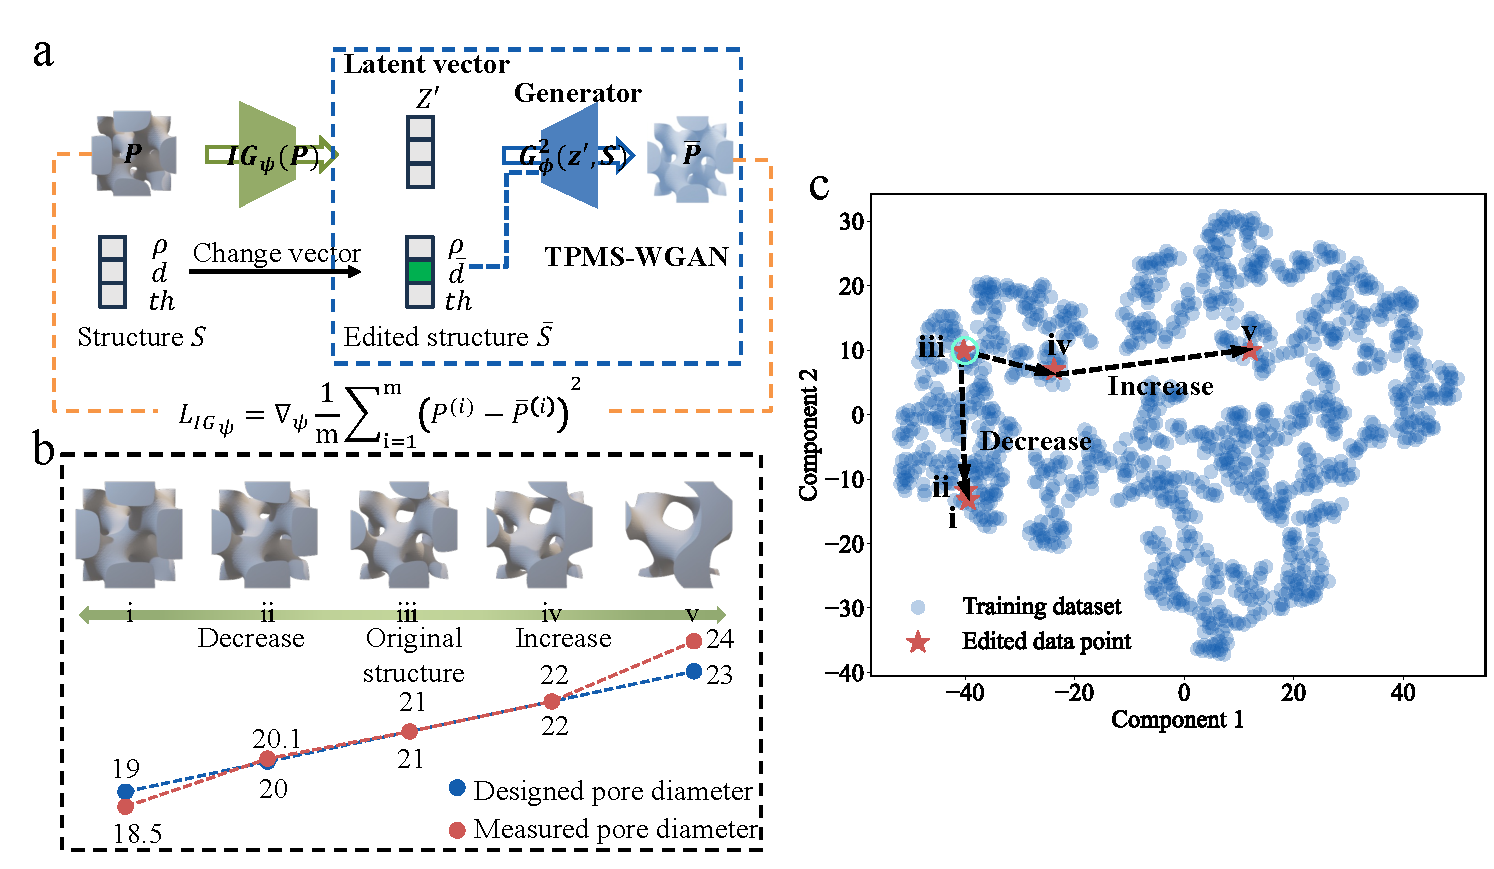
\includegraphics[width=1\linewidth]{figures/5.pdf}
    \caption{\textbf{Inversed TPMS-GAN (ITPMS-GAN) and representative examples of edited geometry of TPMS unit cells. a} The implicit function parameters $\boldsymbol{p}$ of TPMS unit cell with geometry features $\boldsymbol{s}$ are encoded into latent vector $\boldsymbol{z}'$ by ITPMS-GAN ($IG_\psi$). Subsequently, the latent representation $\boldsymbol{z}'$ and edited structure parameters $\bar{\boldsymbol{s}}$ are input to generator $G_\phi^2$ for TPMS unit cell construction. \textbf{b} Geometry evolution of TPMS unit cells is demonstrated through pore diameter variation. Red dots indicate designed pore diameters from ITPMS-GAN, while blue dots represent measured values. \textbf{c} 2D t-SNE plot displays implicit function parameters from training data (blue dots) and five designed TPMS unit cells (red stars). A black dashed line traces the structure evolution path in reduced parameter space.}
    \label{fig:5}
\end{figure}

Bone, a cellular material comprising cortical and cancellous components, exhibits elastic modulus ($E$) values spanning 30-30,000 MPa depending on bone mineral density and demographic factors like age, sex, and race \citep{Wang2016}. While capable of self-repair, critical-sized defects require grafting implants for load support and bone regeneration. For TPMS unit cell applications in bio-implants, two optimization targets emerge: (1) matching scaffold $E$ to native bone modulus to mitigate stress shielding and promote recovery \citep{Yang2020}; (2) maximizing yield strength ($\sigma_{ys}$) for structural integrity.

This study employed TPMS-GAN generator $G_\phi^1$ to produce 100,000 TPMS structures, creating virtual design space $\Omega_E$ targeting 6,000 MPa elastic modulus. As shown in Fig. \ref{fig:6}\textbf{e}, random forest model evaluations revealed generated structure moduli ranging 5,400-6,300 MPa, clustering near the target value (red dashed line). To integrate this target into yield strength active learning, we formulated a constraint function quantifying deviation from 6,000 MPa:

\begin{equation}
    c(\boldsymbol{p}') = 1 - \frac{|E(\boldsymbol{p}') - 6000|}{\max(|E(\boldsymbol{p}') - 6000|)}
\label{eq:22}
\end{equation}

Maximized when $E(\boldsymbol{p}') = 6000$, this constraint function application within the virtual design space is visualized in Fig. \ref{fig:6}\textbf{f}.

\begin{figure}
    \centering
    \includegraphics[width=0.75\linewidth]{figures/6.pdf}
    \caption{\textbf{Schematic of constraint-aware active learning strategy. a} Optimal values and uncertainty predictions for constraint-unaware (\textbf{a1}) versus constraint-aware (\textbf{a2}) approaches. \textbf{b} Next query points determined by Expected Improvement (EI, \textbf{b1}) versus constrained EI (\textbf{b2}). \textbf{c} Virtual design space of TPMS unit cells with 6,000 MPa elastic modulus generated by $G_\phi^1$. \textbf{d} Elastic modulus constraint function implementation in virtual design space.}
    \label{fig:6}
\end{figure}

\subsection{Develop high yield strength TPMS unit cells with matched elastic modulus via the constraint-aware strategy}

Cellular material properties depend on both scaffold architecture and constituent materials, characterized by compressive stress-strain curves. Yield strength ($\sigma_{ys}$), defined at 0.2\% strain, quantifies maximum resistance before irreversible deformation. Computational determination proves resource-intensive due to nonlinear plastic behavior and extensive meshing requirements. TPMS unit cell yield strength simulations require approximately 30 minutes per sample, whereas elastic modulus evaluation via finite element homogenization takes roughly 1 minute (computational details in Supplementary Note S6). Bayesian optimization efficiently addresses such expensive black-box problems.

Our constraint-aware active learning approach optimizes yield strength while maintaining elastic modulus targets. A support vector machine (SVM) serves as surrogate model, with bootstrap resampling assessing uncertainties through replacement sampling. Initial implementation sampled 16 candidates from virtual design space for FEM yield strength evaluation. SVM training involved 50 iterations producing resampled training sets and corresponding models. Each initial sample generated 50 predictions used to calculate mean ($\mu$) and standard deviation ($\Sigma$).

Figure \ref{fig:7}c demonstrates constraint-aware Expected Improvement shifting query samples from blue to red dots in the first iteration (Section \ref{sec:2-4}). This transition reflects elastic modulus constraints modifying expected improvement relative to training dataset maxima. Four iterations were conducted, with two samples evaluated per iteration for subsequent feedback into the learning cycle.


The diagonal plot in Fig \ref{fig:7}\textbf{a} demonstrates that model predictions largely align with observed values. The constraint-aware active learning strategy successfully recommends samples exhibiting high yield strength. We track mean square error (MSE) and $R^2$ metrics as the surrogate model undergoes iterative refinement through evaluation of TPMS structures, as shown in Fig \ref{fig:7}\textbf{b}.

The elastic modulus and yield strength distributions of recommended samples are presented in Figs. \ref{fig:7}d-e. Analysis reveals that these samples exhibit elastic moduli clustered near 6,000 MPa, with a mean value of approximately 5,900 MPa – notably higher than the initial dataset's mean of 5,800 MPa. Furthermore, yield strength values for recommended samples consistently exceed those in the initial dataset.

To quantify overall performance $Y$ of TPMS unit cells under the constraint-aware active learning framework, we employ:

\begin{equation}
    Y = Y_E^N + Y_{\sigma_{ys}}^N \label{eq:23}
\end{equation}

where

\begin{equation}
\begin{aligned}
Y_E^N &= \frac{Y_E - \min(Y_E)}{\max(Y_E) - \min(Y_E)}, & Y_E &= \frac{1}{|E(\boldsymbol{p}') - E^*|} \\
Y_{\sigma_{ys}}^N &= \frac{Y_{\sigma_{ys}} - \min(Y_{\sigma_{ys}})}{\max(Y_{\sigma_{ys}}) - \min(Y_{\sigma_{ys}})}
\end{aligned}
\label{eq:24}
\end{equation}

This composite metric effectively quantifies TPMS unit cell performance in achieving scaffold designs with matched elastic modulus and enhanced yield strength. Fig \ref{fig:7}g shows peak performance ($Y$ = 1.72) occurring at iteration 2, significantly surpassing the initial dataset's optimal value (0.22). A transient performance decrease at iteration 3 reflects the active learning process balancing exploration and exploitation strategies, with subsequent recovery to improved performance by iteration 4.

Stress analysis reveals localized concentration at unit cell junctions, as demonstrated in the von Mises stress cloud plot (Fig \ref{fig:7}h) and stress-strain curve (Fig \ref{fig:7}i). The constraint-aware active learning method exhibits extrapolation capability, identifying optimal TPMS structures beyond training data distributions – a critical advantage for clinical applications where patient-specific target properties and initial data variability present challenges.

Implementation of this framework reduces design costs substantially, requiring only 24 yield strength assessments compared to 1,372 evaluations needed for traditional bi-objective generative model training. This efficiency gain translates to an approximately sixfold reduction in design time.

\begin{figure}
    \centering
    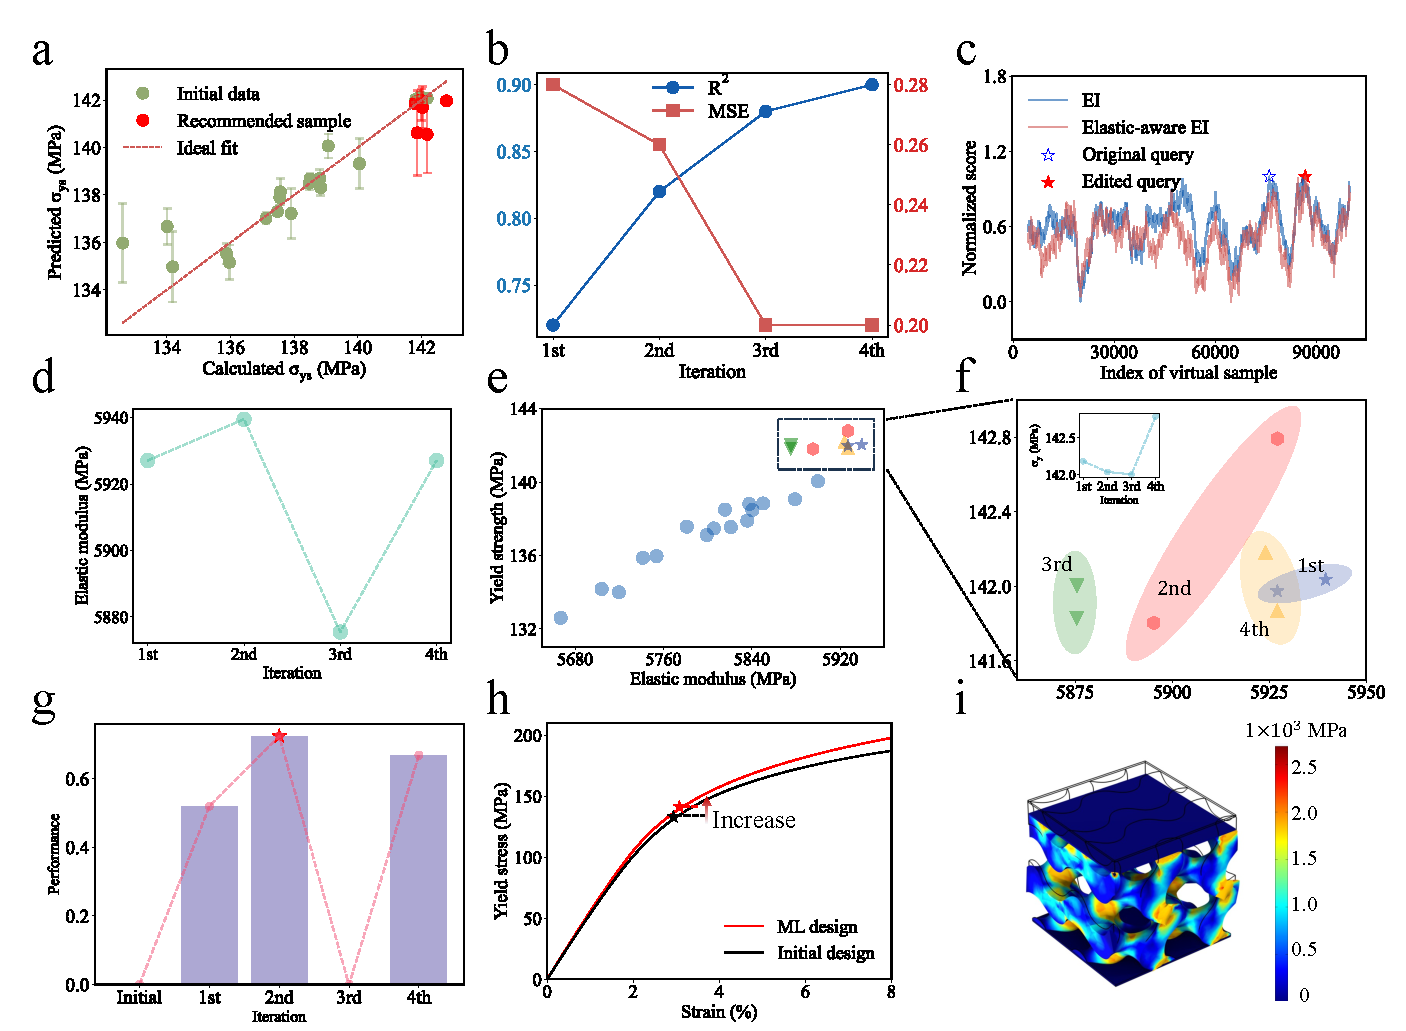
\includegraphics[width=1\linewidth]{figures/7.pdf}
    \caption{\textbf{Active learning workflow for yield stress optimization of TPMS unit cells under elastic modulus constraints. a} SVM diagonal plot: recommended structures (red) versus initial data (green). \textbf{b} Iterative improvement of SVM regressor performance. \textbf{c} Query point comparison between EI and constraint-aware EI at iteration 1. \textbf{d} Elastic modulus evolution across iterations. \textbf{e} Yield strength-elastic modulus distributions: recommended samples vs initial data (blue). \textbf{f} Parameter progression through active learning iterations. \textbf{g} Overall performance trajectory. \textbf{h} Stress-strain curves: optimal recommended structure versus initial dataset optimum. \textbf{i} von Mises stress distribution in the recommended optimal structure.}
    \label{fig:7}
\end{figure}

\section{Conclusions}
This study presents a data-efficient, two-stage bi-objective inverse design methodology for TPMS-based orthopedic implants, integrating generative modeling, active learning, and finite element analysis while addressing cost disparities between objectives. The framework simultaneously optimizes:
1) Elastic modulus matching to bone tissue for stress-shielding mitigation
2) Yield strength maximization for mechanical stability

Cubic symmetric TPMS unit cells (G/D) were combined to create isotropic cellular materials, with effective elastic tensors calculated via voxel-based numerical homogenization. Our TPMG-GAN architecture generates target-specific virtual structures through navigator-guided synthesis, while the ITPMS-GAN variant enables explainable geometric feature-to-structure mapping without latent space interpolation or implicit function adjustment. These approaches expand design possibilities for TPMS architectures.

The constraint-aware active learning framework achieved a remarkable performance improvement from 0.2 to 1.7 compared to initial datasets, demonstrating extrapolation capability beyond training data distributions. Combined with sixfold acceleration in design efficiency, this methodology provides robust solutions for clinical scenarios involving variable patient-specific requirements and uncertain mechanical property ranges.

\section*{CRediT authorship contribution statement}
Jiaxuan Ma: Writing – original draft, Software, Methodology, Investigation, Formal analysis, Conceptualization. Bin Cao: Software, Investigation, Conceptualization, Formal analysis. Yuan Tian: Writing – review \& editing, Investigation, Formal analysis. Sheng Sun: Writing – review \& editing, Supervision, Funding acquisition, Formal analysis.

\section*{Declaration of competing interest}
The authors declare that they have no known competing financial interests or personal relationships that could have appeared to influence the work reported in this paper.

%% The Appendices part is started with the command \appendix;
%% appendix sections are then done as normal sections
%% \appendix
%% \section{}
%% \label{}
%% If you have bibdatabase file and want bibtex to generate the
%% bibitems, please use
%%
\bibliographystyle{elsarticle-harv} 
\bibliography{refs}
%% else use the following coding to input the bibitems directly in the
%% TeX file.
% \begin{thebibliography}{00}
% %% \bibitem[Author(year)]{label}
% %% Text of bibliographic item
% \bibitem[ ()]{}
% \end{thebibliography}
\end{document}
\endinput
%%
%% End of file `elsarticle-template-harv.tex'.'
